\section{状态转移与多步分布}
\label{sec:dtsp-transitions}

本节回答一个基础问题：只知道“下一步怎样从当前状态产生”，能否算出整条随机序列的联合规律，特别是若干步以后的分布。我们先从可以直接执行的随机递推出发，说明Markov性质从哪里来；再用转移矩阵和转移核把一步规律写成可以复合的对象。全章以$n\in\mathbb N_0=\{0,1,2,\ldots\}$表示时刻，状态空间记为可测空间$(E,\mathcal E)$；$E$可数时用$i,j$表示状态。滤过$(\mathcal F_n)_{n\geq0}$表示到时刻$n$为止可用的信息，其定义与适应性沿用第~\ref{chap:stochastic-processes-and-sample-paths}章。

\subsection{随机递推与Markov性质}
\label{sec:dtsp-random-recursion}

\paragraph{由噪声驱动的递推}
最容易执行的随机序列是在确定性更新中加入新噪声：
\begin{equation}
  X_{n+1}=F(X_n,\xi_{n+1}),\qquad n\geq0,
  \label{eq:dtsp-random-recursion}
\end{equation}
其中$F:E\times U\to E$可测，$\xi_1,\xi_2,\ldots$取值于可测空间$U$，相互独立且同分布，并与初态$X_0$独立。每一步只需要当前状态和一份新抽取的噪声，计算机可以逐步模拟整条路径。

把很多条路径画在同一张图上，可以同时看见“一条实现”和“一个分布”。取$E=\mathbb R$、$F(x,\xi)=0.8x+\xi$、$\xi_n\sim\mathcal N(0,1)$，从$X_0=4$出发。图~\ref{fig:dtsp-ar1-path-bundle}(a)中每条细线是一次实现；固定某个时刻$n$竖直切一刀，切口上的点云就是$X_n$的分布。由递推取期望和方差，
\[
  \mathbb EX_n=4\times0.8^n,\qquad
  \operatorname{Var}(X_n)=\sum_{k=0}^{n-1}0.64^k=\frac{1-0.64^n}{0.36},
\]
因为$X_n=0.8^nX_0+\sum_{k=1}^{n}0.8^{n-k}\xi_k$是独立高斯变量的线性组合。均值以$0.8^n$的速度回到零，方差则增长到$1/0.36\approx2.78$后不再变化；图(b)显示$X_1,X_3,X_{10}$的密度逐渐靠近同一条极限曲线。

\begin{figure}[htbp]
  \centering
  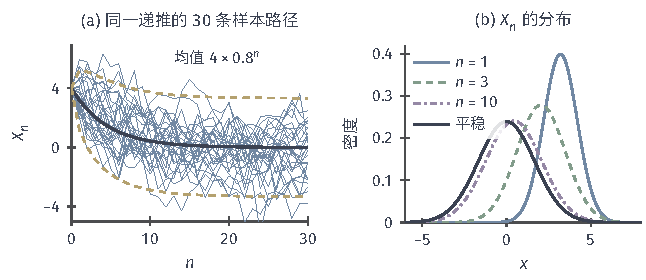
\includegraphics[width=107mm]{figures/03-optimization-evolution-and-signals/02-processes-and-trajectory-evolution/tikz/dtsp-ar1-path-bundle/figure.pdf}
  \caption{随机递推$X_{n+1}=0.8X_n+\xi_{n+1}$的路径束与边缘分布。$\xi_n$独立服从$\mathcal N(0,1)$，$X_0=4$。(a)30条模拟路径（固定随机种子），黑线为精确均值$4\times0.8^n$，黄色虚线为均值加减两倍精确标准差；(b)$n=1,3,10$时$X_n$的精确高斯密度，黑线为极限分布$\mathcal N(0,1/0.36)$。}
  \label{fig:dtsp-ar1-path-bundle}
\end{figure}

现在问：已知到时刻$n$的全部历史，下一状态的条件分布是什么？给定$\mathcal F_n=\sigma(X_0,\xi_1,\ldots,\xi_n)$后，$X_n$已经确定，而$\xi_{n+1}$与$\mathcal F_n$独立。条件期望的代入法则（可参考\BookChapterRef{chap:conditional-expectation}{卷二“条件期望与条件分布”章}）允许把已知的$X_n$当作常数代入，再对独立的$\xi_{n+1}$求平均：对每个$B\in\mathcal E$，
\begin{equation}
  \mathbb P(X_{n+1}\in B\mid\mathcal F_n)
  =\mathbb P\bigl(F(x,\xi_{1})\in B\bigr)\big|_{x=X_n}
  \qquad\text{几乎必然}.
  \label{eq:dtsp-recursion-conditional-law}
\end{equation}
右侧只通过$X_n$依赖历史。也就是说，当前状态已经把预测下一步所需的全部历史信息概括起来了。下面把这个性质单独定义，因为它不依赖于具体的递推写法。

\begin{definition}[Markov性质]
  \label{def:dtsp-markov-property}
  设过程$(X_n)_{n\geq0}$取值于$(E,\mathcal E)$并适应于滤过$(\mathcal F_n)$。若对每个$n\geq0$和每个$B\in\mathcal E$，
  \[
    \mathbb P(X_{n+1}\in B\mid\mathcal F_n)=\mathbb P(X_{n+1}\in B\mid X_n)\qquad\text{几乎必然},
  \]
  则称$(X_n)$相对于$(\mathcal F_n)$具有Markov性质，称它为\term{Markov链}（Markov chain）。未指明滤过时取自然滤过$\mathcal F_n=\sigma(X_0,\ldots,X_n)$。
\end{definition}

定义中的条件$\sigma$代数不可省略。若把滤过放大为$\mathcal G_n=\sigma(X_0,\xi_1,\ldots,\xi_{n+1})$，即提前一步知道下一份噪声，那么$X_{n+1}=F(X_n,\xi_{n+1})$对$\mathcal G_n$已经可测，它给定$\mathcal G_n$的条件分布是点质量，而给定$X_n$的条件分布仍然分散，Markov等式不再成立。同一组随机变量相对于不同的信息流可以有不同的结论；这也是第~\ref{chap:stochastic-processes-and-sample-paths}章强调先声明滤过的原因。

\paragraph{当前读数不够时扩充状态}
Markov性质是对“状态”选得是否充分的检验。考虑二阶递推
\[
  Y_{n+1}=1.2Y_n-0.5Y_{n-1}+\xi_{n+1},
\]
其中$\xi_n$独立同分布于$\mathcal N(0,1)$，并与$(Y_0,Y_1)$独立。给定$(Y_n,Y_{n-1})$时，$Y_{n+1}$的条件均值是$1.2Y_n-0.5Y_{n-1}$，显式依赖上一时刻。若$(Y_n)$本身相对于自然滤过是Markov链，给定全部历史的条件均值就只能是$Y_n$的函数；而给定$Y_n$后$Y_{n-1}$通常仍有正的条件方差，$-0.5Y_{n-1}$这一项无法写成$Y_n$的函数。因此仅记录当前读数不足以预测下一步。

补救办法是把仍然影响未来的历史放进状态。令$\bm Z_n=(Y_n,Y_{n-1})^{\top}$，则
\[
  \bm Z_{n+1}=
  \begin{pmatrix}1.2&-0.5\\1&0\end{pmatrix}\bm Z_n
  +\begin{pmatrix}\xi_{n+1}\\0\end{pmatrix},
\]
这正是式~\eqref{eq:dtsp-random-recursion}的形式，于是$(\bm Z_n)$是Markov链。相关噪声也可以这样处理：若$Y_{n+1}=0.8Y_n+\eta_{n+1}$而$\eta_{n+1}=0.5\eta_n+\xi_{n+1}$，则$(Y_n,\eta_n)$构成Markov状态。扩充状态的代价是维数增加；它把“历史依赖”改写为“高维状态的当前值依赖”，并不消除依赖本身。

\paragraph{时间齐次不等于分布不变}
在式~\eqref{eq:dtsp-random-recursion}中，更新映射$F$和噪声分布都不随$n$改变，因此每一步的条件规律相同。这种性质称为\term{时间齐次的}（time-homogeneous）。它说的是“规则不变”，而不是“分布不变”：图~\ref{fig:dtsp-ar1-path-bundle}中的递推是时间齐次的，但从$X_0=4$出发时$X_n$的均值和方差一直在变。规则不变时分布能否最终稳定、稳定到哪里，是第~\ref{sec:dtsp-long-run}节研究的问题。

\subsection{转移矩阵与转移核}
\label{sec:dtsp-kernels}

\paragraph{有限状态：转移矩阵}
先看状态有限的情形。设一台服务器每秒处于“正常”（状态$1$）或“拥堵”（状态$2$）之一。若当前正常，下一秒以$0.1$的概率变为拥堵；若当前拥堵，下一秒以$0.2$的概率恢复。把条件概率排成矩阵，
\begin{equation}
  \bm P=\begin{pmatrix}P_{1,1}&P_{1,2}\\P_{2,1}&P_{2,2}\end{pmatrix}
  =\begin{pmatrix}0.9&0.1\\0.2&0.8\end{pmatrix},
  \qquad P_{i,j}=\mathbb P(X_{n+1}=j\mid X_n=i).
  \label{eq:dtsp-two-state-matrix}
\end{equation}
图~\ref{fig:dtsp-two-state-graph}把它画成有向图：每个节点的出边概率之和为一。这条两状态链将作为全章的贯穿例子。

\begin{figure}[htbp]
  \centering
  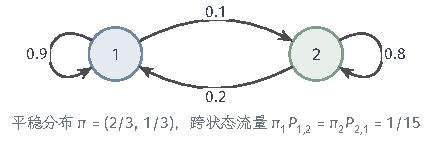
\includegraphics[width=73mm]{figures/03-optimization-evolution-and-signals/02-processes-and-trajectory-evolution/tikz/dtsp-two-state-graph/figure.pdf}
  \caption{两状态链的转移图。节点为状态，带箭头的边标出一步转移概率，自环表示停留；每个状态的出边概率之和为$1$。图下说明的平稳分布与概率流将在第~\ref{sec:dtsp-invariant}节和第~\ref{sec:dtsp-reversibility}节导出。}
  \label{fig:dtsp-two-state-graph}
\end{figure}

一般地，可数状态集$E$上的矩阵$\bm P=(P_{i,j})$若满足$P_{i,j}\geq0$且每行之和$\sum_jP_{i,j}=1$，称为\termalias{stochastic-matrix}{随机矩阵}（stochastic matrix）。时间齐次Markov链的转移矩阵就是这样的矩阵。它与初始分布$\bm\mu$一起确定一段路径的概率：
\begin{equation}
  \mathbb P(X_0=i_0,X_1=i_1,\ldots,X_n=i_n)=\mu_{i_0}P_{i_0,i_1}P_{i_1,i_2}\cdots P_{i_{n-1},i_n}.
  \label{eq:dtsp-path-probability}
\end{equation}
推导只用乘法公式：联合概率等于$\mathbb P(X_0=i_0)$依次乘以各步给定此前全部状态的条件概率，而Markov性质把第$k$个条件概率化为$P_{i_{k-1},i_k}$。例如从正常状态出发，“正常、正常、拥堵、拥堵”这段路径的概率是$1\times0.9\times0.1\times0.8=0.072$。

把式~\eqref{eq:dtsp-path-probability}对中间状态求和，就得到下一步的分布。把分布写成行向量$\bm\mu_n^{\top}=(\mathbb P(X_n=i))_{i\in E}$，则
\[
  \bm\mu_{n+1}^{\top}=\bm\mu_n^{\top}\bm P,\qquad
  \bm\mu_n^{\top}=\bm\mu_0^{\top}\bm P^n.
\]
从$\bm\mu_0=(1,0)^{\top}$出发，前两步是$(0.9,0.1)$与$(0.9\times0.9+0.1\times0.2,\;0.9\times0.1+0.1\times0.8)=(0.83,0.17)$。

\paragraph{一般状态：转移核}
状态取实数时，单点的概率通常为零，不能再列出矩阵。替代对象是对每个当前状态给出一个下一步分布的映射。

\begin{definition}[转移核]
  \label{def:dtsp-transition-kernel}
  映射$P:E\times\mathcal E\to[0,1]$若满足：对每个$x\in E$，$B\mapsto P(x,B)$是$(E,\mathcal E)$上的概率测度；对每个$B\in\mathcal E$，$x\mapsto P(x,B)$可测，则称$P$为$E$上的\term{转移核}（transition kernel）。若对所有$n\geq0$和$B\in\mathcal E$都有
  \[
    \mathbb P(X_{n+1}\in B\mid\mathcal F_n)=P(X_n,B)\qquad\text{几乎必然},
  \]
  则称$(X_n)$是相对于$(\mathcal F_n)$、以$P$为转移核的时间齐次Markov链。
\end{definition}

第一项要求说每个状态都对应一个合法的下一步分布。第二项可测性的用途在于对随机的当前状态积分：若$X_n\sim\mu_n$，则
$\mathbb P(X_{n+1}\in B)=\mathbb E[P(X_n,B)]=\int_EP(x,B)\,\mu_n(\mathrm dx)$，而这个积分只对可测函数有定义。递推~\eqref{eq:dtsp-random-recursion}给出的核是$P(x,B)=\mathbb P(F(x,\xi_1)\in B)$；在图~\ref{fig:dtsp-ar1-path-bundle}的例子中，$P(x,\cdot)=\mathcal N(0.8x,1)$。第~\ref{chap:stochastic-processes-and-sample-paths}章已经说明，给定初始分布和转移核，可以在路径空间上构造出相应的过程；本章直接使用这个过程。

\paragraph{核作用于分布与作用于函数}
同一个核有两种用法，分别对应“分布向前推”和“函数向后拉”。对概率测度$\mu$和有界可测函数$f$，定义
\begin{equation}
  (\mu P)(B)=\int_E P(x,B)\,\mu(\mathrm dx),\qquad
  Pf(x)=\int_E f(y)\,P(x,\mathrm dy).
  \label{eq:dtsp-kernel-actions}
\end{equation}
$\mu P$是从分布$\mu$出发走一步后的分布；$Pf(x)$是从$x$出发走一步后$f$的平均值，即$\mathbb E[f(X_{n+1})\mid X_n=x]$。两种作用由
\[
  (\mu P)f=\int f\,\mathrm d(\mu P)=\int Pf\,\mathrm d\mu=\mu(Pf)
\]
联系起来，等式由Fubini定理对非负或有界函数成立。有限状态时，$\mu P$是行向量乘矩阵，$Pf$是矩阵乘列向量。区分两者很有用：研究分布怎样演化时用$\mu P$，研究条件期望和鞅时用$Pf$。

\paragraph{多步转移与Chapman--Kolmogorov关系}
两个核$P,Q$的复合定义为
\[
  (PQ)(x,B)=\int_E Q(y,B)\,P(x,\mathrm dy),
\]
它表示先按$P$走一步、再按$Q$走一步。令$P^0(x,B)=\mathbb I\{x\in B\}$，$P^{m+1}=P^mP$。下面的定理说明核的幂恰好给出多步转移。

\begin{theorem}[多步转移与Chapman--Kolmogorov关系]
  \label{thm:dtsp-chapman-kolmogorov}
  设$(X_n)$是以$P$为转移核的时间齐次Markov链。则对所有$n,m\geq0$和有界可测$f$，
  \begin{equation}
    \mathbb E[f(X_{n+m})\mid\mathcal F_n]=P^mf(X_n)\qquad\text{几乎必然},
    \label{eq:dtsp-multistep}
  \end{equation}
  并且核的幂满足
  \begin{equation}
    P^{m+k}(x,B)=\int_EP^k(y,B)\,P^m(x,\mathrm dy),\qquad x\in E,\ B\in\mathcal E.
    \label{eq:dtsp-chapman-kolmogorov}
  \end{equation}
\end{theorem}

\begin{proof}
对$m$归纳证明式~\eqref{eq:dtsp-multistep}。$m=0$时两边都是$f(X_n)$。设结论对$m$成立。由塔式性质先对$\mathcal F_{n+m}$取条件期望，
\[
  \begin{aligned}
    \mathbb E[f(X_{n+m+1})\mid\mathcal F_n]
    &=\mathbb E\bigl[\mathbb E[f(X_{n+m+1})\mid\mathcal F_{n+m}]\bigm|\mathcal F_n\bigr]\\
    &=\mathbb E[Pf(X_{n+m})\mid\mathcal F_n].
  \end{aligned}
\]
第二个等号用了转移核的定义（先对指示函数成立，再由线性与单调收敛推广到有界可测$f$）。$Pf$仍有界可测，对它使用归纳假设得到$P^m(Pf)(X_n)=P^{m+1}f(X_n)$。式~\eqref{eq:dtsp-chapman-kolmogorov}是核复合的结合律：$P^{m+k}=P^mP^k$，按复合的定义展开即得。
\end{proof}

式~\eqref{eq:dtsp-chapman-kolmogorov}称为\term{Chapman--Kolmogorov关系}，它的含义是：从$x$走$m+k$步到$B$，可以先任意走$m$步到某个中间状态$y$，再从$y$走$k$步，按中间状态的分布平均。有限状态时它就是矩阵乘法$\bm P^{m+k}=\bm P^m\bm P^k$。

\paragraph{两状态链的多步分布}
对矩阵~\eqref{eq:dtsp-two-state-matrix}，可以显式算出$\bm P^n$。它的右特征向量为$(1,1)^{\top}$（特征值$1$）和$(1,-2)^{\top}$（特征值$0.7$），后者可直接验证：$\bm P(1,-2)^{\top}=(0.7,-1.4)^{\top}$。按这组特征向量展开得到
\begin{equation}
  \bm P^n=
  \begin{pmatrix}2/3&1/3\\2/3&1/3\end{pmatrix}
  +0.7^n\begin{pmatrix}1/3&-1/3\\-2/3&2/3\end{pmatrix}.
  \label{eq:dtsp-two-state-power}
\end{equation}
$n=1$时右侧确实回到$\bm P$。令$q_n=\mathbb P(X_n=2)$，一步关系为$q_{n+1}=0.1(1-q_n)+0.8q_n=0.1+0.7q_n$，于是
\[
  q_n=\frac13+0.7^n\Bigl(q_0-\frac13\Bigr).
\]
从正常状态出发，$q_1=0.1$、$q_2=0.17$、$q_{10}\approx0.324$。图~\ref{fig:dtsp-two-state-distribution}(a)画出从两个初态出发的$q_n$：两条曲线都以$0.7^n$的速度靠近$1/3$，但没有任何一步恰好等于它。式~\eqref{eq:dtsp-two-state-power}已经预告了后面几节的主题：第一项是被转移保持的分布，第二项是逐步衰减的初态影响，而衰减率$0.7=1-0.1-0.2$由两种跳转概率共同决定。

\begin{figure}[htbp]
  \centering
  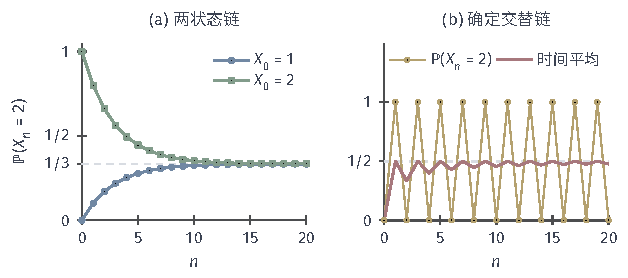
\includegraphics[width=106mm]{figures/03-optimization-evolution-and-signals/02-processes-and-trajectory-evolution/tikz/dtsp-two-state-distribution/figure.pdf}
  \caption{多步分布的两种长期表现（精确计算）。(a)两状态链~\eqref{eq:dtsp-two-state-matrix}从状态$1$和状态$2$出发时的$\mathbb P(X_n=2)=1/3+0.7^n(q_0-1/3)$，虚线为$1/3$；(b)确定交替链（$1\to2\to1\to\cdots$）从状态$1$出发时，$\mathbb P(X_n=2)$在$0,1$之间交替，红线为前$n+1$个时刻的平均，趋于$1/2$。}
  \label{fig:dtsp-two-state-distribution}
\end{figure}
